\subsection{AGRC analysis}
\label{sec:agrc-analysis}

%In order to statically determine the worst case memory consumption of a
%program targeting TP-JOP, one needs to analyze codes generated from both
%CNs and JDNs. The compiler is able to trivially determine the maximum
%memory footprint required for executing CN codes from any given SystemJ
%programs [] since there is no dynamic memory allocation required for
%executing this code. On the other hand, the data-flow analysis for JDNs
%is more intricate since it needs to analyze the original AGRC in order
%to retrieve the dependency edges, which are lost after splitting CNs and
%JDNs from the AGRC. We devote this section to illustrate this analysis
%technique.


AGRC is a \textit{directed graph} of tuple $G =(V,E)$, where $V$ is the
set of vertices (nodes of AGRC) and $E$ is the set of ordered pairs of
vertices. Each edge $e = (v_i,v_j), \forall e \in E, v_i \in V, v_j \in
V$ is a tuple denoting that the edge is directed from $v_i$ to $v_j$.
Then a lambda  function $\lambda:v \rightarrow E_i$, $E_i \subseteq E$,
maps \textit{each} vertex to a set of edge(s) where $\forall (v_i,v_j)
\in E_i, v_j = v$ and $E_i$ can be $\emptyset$. When $|E_i| = 1$ we call
$v_i$ \textit{must} be called before $v$ whereas when $|E_i| > 1$ we
call any $v_i \in E_i$ \textit{may} be called before $v$.

\begin{figure}[t!]
	\newsavebox{\codeone}
	\begin{lrbox}{\codeone}
		\begin{minipage}[b]{0.62\textwidth}
		\begin{lstlisting}[tabsize=1,basicstyle=\small\ttfamily,numbers=left]
(mList 
	(mNode JDN1 (Must Null) (May Null))
	(mNode JDN2 
		(Must (mNode JDN1 (Must Null) (May Null))) 
		(May Null))
	(mNode JDN3 
		(Must (mNode JDN1 (Must Null) (May Null))) 
		(May Null))
	(mNode JDN4 (Must Null)
		(May 
			(mNode JDN2 
				(Must (mNode JDN1 (Must Null) (May Null))) 
				(May Null))
			(mNode JDN3 
				(Must (mNode JDN1 (Must Null) (May Null))) 
				(May Null))))
		\end{lstlisting}
	\end{minipage}
	\end{lrbox}

	\centering
	\subfloat[An abstracted AGRC graph]{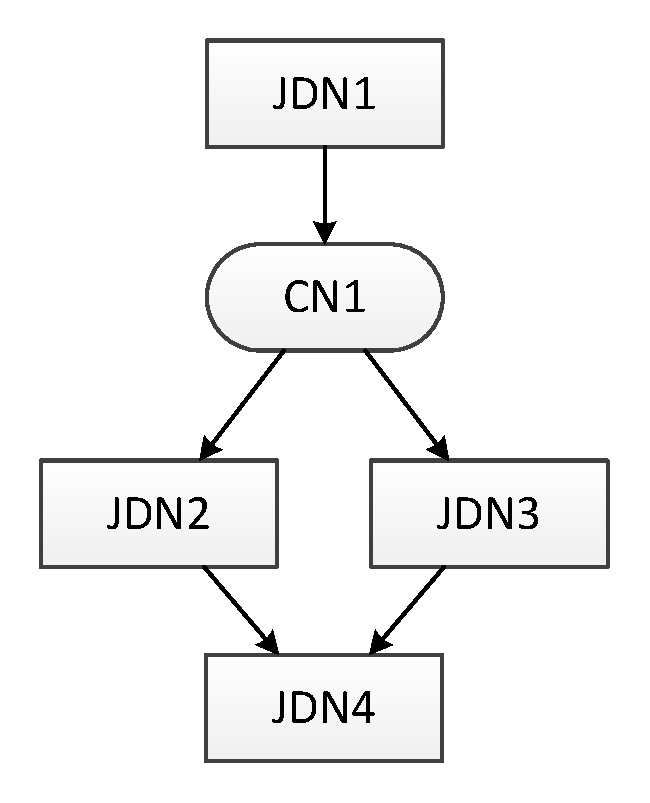
\includegraphics[scale=0.3]{may}
	\label{fig:aagrc}}
	\hspace{1.0cm}
	\subfloat[An output of the AGRC
	analysis]{\scalebox{0.8}{\usebox{\codeone}}\label{fig:tttt}}
	\caption{An example of AGRC analysis}
	\label{fig:maymust}
\end{figure}

In this section, we illustrate how a data-structure, which contains
information on the \textit{may} and \textit{must} relationships between
the nodes, is obtained from the AGRC. Consider a snippet of AGRC graph
shown in Figure~\ref{fig:aagrc}. Here, a root node, \texttt{JDN1}, has
no parent whereas it has an immediate child \texttt{CN1}. \texttt{CN1}
has two children, \texttt{JDN2} and \texttt{JDN3}, and both of these
JDNs have an identical child \texttt{JDN4}. A result of the analysis of
this graph is shown in Figure~\ref{fig:tttt}, which is written in
S-expression format. An output of the analysis is a set of nodes called
\texttt{mNode}. \texttt{mNode} has three fields, a node name of type
string, \texttt{Must} of type \texttt{mNode} and \texttt{May} of a set
of type \texttt{mNode}. Our analysis tool then use this data-structure
to identify potential callers of each \texttt{JDN}. For instance, since
\texttt{JDN1} has no parents, its \texttt{Must} and \texttt{May} fields
are both \texttt{Null} (line 2).  On the other hand, \texttt{JDN1} must
be calling \texttt{JDN2} or \texttt{JDN3}, hence \texttt{Must} of both
\texttt{JDN2} and \texttt{JDN3} is \texttt{JDN1} (lines 4 and 7).
Lastly, \texttt{JDN4} has two parent nodes; \texttt{JDN2} and
\texttt{JDN3}. Therefore, its \texttt{May} field has both \texttt{JDN2}
and \texttt{JDN3} (lines 11-16). It should be noted that we are only
interested in callers of \texttt{JDNs}, hence \texttt{CNs} are not
included in the final result (Figure~\ref{fig:tttt}). A complete
algorithm of our AGRC analysis is shown in Appendix~\ref{ap:1}.






%%% Local Variables:
%%% mode: latex
%%% TeX-master: "jgc"
%%% End:
